\section{Sets}

\subsection{Why sets are the grammar of modern mathematics}

A set is one of the first ideas in rigorous mathematics that feels both too simple and too slippery. Too simple, because a set is just a collection of objects. Too slippery, because that sentence hides nearly everything that later mathematics needs: membership, equality, containment, construction, size, structure, and the discipline of saying exactly what kind of object we are talking about.

When we say
\[
A=\{1,2,3\},
\]
we are not naming three numbers separately. We are naming one object whose members are the numbers $1$, $2$, and $3$. This shift is small but powerful. A set lets us treat many things as one thing.

That is already familiar from software. A list, array, database table, hash set, type, interface, and collection all let us talk about many possible values as a single object. But mathematical sets are not arrays. A set has no order and no repeated entries. The set $\{1,2,3\}$ is the same set as $\{3,2,1\}$ and as $\{1,1,2,3,3\}$.

\begin{focusbox}
A set is determined by its members, not by how those members are written down.
\end{focusbox}

The membership symbol
\[
x\in A
\]
means that $x$ is an element of $A$. Its negation
\[
x\notin A
\]
means that $x$ is not an element of $A$.

The statement $2\in\{1,2,3\}$ is true. The statement $4\in\{1,2,3\}$ is false. The statement $\{2\}\in\{1,2,3\}$ is false, because $\{2\}$ is a set, not the number $2$.

\begin{trapbox}
Do not confuse an object with a set containing that object. Usually $2\neq\{2\}$. The first is a number. The second is a set whose only member is that number.
\end{trapbox}

Sets become essential because most later definitions begin by saying what kind of objects are allowed. A function has a domain and codomain, both sets. A sequence is a function whose domain is often $\N$. A metric space is a set equipped with a distance function. A group is a set equipped with an operation. A topological space is a set equipped with a collection of open subsets. A vector space is a set equipped with addition and scalar multiplication.

That pattern is worth noticing:
\[
\text{mathematical structure}=\text{set}+\text{extra data}+\text{rules}.
\]

Before we can understand the extra data, we need to understand the set underneath it.

\subsection{Membership, equality, and extensionality}

The most basic relation between an object and a set is membership. The most basic relation between two sets is equality.

\begin{formalbox}
Two sets $A$ and $B$ are equal if and only if they have exactly the same elements:
\[
A=B \quad\Longleftrightarrow\quad \forall x,\ (x\in A\Longleftrightarrow x\in B).
\]
\end{formalbox}

This principle is called extensionality. It says that a set is determined by its extension, meaning the objects that belong to it.

For example,
\[
\{n\in\Z:n^2=1\}=\{-1,1\}.
\]
The left side describes the set by a property. The right side lists its elements. They are the same set because they contain the same objects.

This is also why order and repetition do not matter:
\[
\{a,b,c\}=\{c,a,b\}=\{a,a,b,c,c\}.
\]
All three have the same members.

\begin{intuitionbox}
A set is like a yes-or-no test for membership. For each object $x$ under discussion, the set $A$ answers: yes, $x\in A$, or no, $x\notin A$.
\end{intuitionbox}

That membership-test perspective will later connect directly to logic and software. A subset of a universe $U$ can be represented by a Boolean-valued predicate on $U$. If $A\subseteq U$, then $A$ corresponds to the predicate
\[
P_A(x): x\in A.
\]
In a program, this might be a function returning true or false. In mathematics, it is a property that determines membership.

The phrase ``under discussion'' matters. In ordinary set theory, membership is not restricted to one universal type. But in actual proofs, we almost always work inside a domain: integers, real numbers, functions, matrices, points in a space, ideals in a ring. Your proof becomes clearer when you keep that ambient universe visible.

\begin{walkbox}
Pick a set you know, such as $\Z$, $\Q$, or the set of continuous functions $\R\to\R$. Ask: what counts as an element of this set, and what would be a thing that looks related but is not an element?
\end{walkbox}

\subsection{Roster notation and set-builder notation}

There are two common ways to specify sets. Roster notation lists members:
\[
A=\{2,4,6,8\}.
\]
Set-builder notation describes members by a condition:
\[
B=\{n\in\Z: n \text{ is even and }2\leq n\leq 8\}.
\]
Here $A=B$.

Set-builder notation has the general shape
\[
\{x\in D:P(x)\},
\]
read as ``the set of all $x$ in $D$ such that $P(x)$.''

The domain $D$ is not decoration. Compare:
\[
\{x\in\R:x^2<2\}
\]
with
\[
\{x\in\Z:x^2<2\}.
\]
The first is the interval $(-\sqrt2,\sqrt2)$. The second is $\{-1,0,1\}$. The formula $x^2<2$ did not change, but the set changed because the allowed inputs changed.

\begin{trapbox}
The expression $\{x:x^2<2\}$ is often understandable from context, but it is dangerous when no universe is clear. In early proof writing, include the domain.
\end{trapbox}

Set-builder notation also trains you to read quantifiers. The statement
\[
y\in\{x\in D:P(x)\}
\]
means exactly:
\[
y\in D\text{ and }P(y).
\]
Nothing mystical happens inside the braces. The bound variable $x$ is local. We could write
\[
\{t\in D:P(t)\}
\]
and get the same set.

Examples:
\[
\{n\in\N:n\leq 5\}=\{1,2,3,4,5\}
\]
if $\N=\{1,2,3,\ldots\}$.
\[
\{x\in\R:x^2+1=0\}=\varnothing.
\]
\[
\{z\in\C:z^2+1=0\}=\{i,-i\}.
\]

The last two examples are a useful warning. A set can be empty in one universe and nonempty in another. Algebra, analysis, and geometry often differ precisely because they change the universe.

\subsection{The empty set and singleton sets}

The empty set is the set with no elements. It is written
\[
\varnothing.
\]
It is not nothing. It is a set. It is the unique set satisfying
\[
\forall x,\ x\notin\varnothing.
\]

This can feel pedantic, but the empty set behaves like zero in arithmetic. It is the identity for union:
\[
A\cup\varnothing=A.
\]
It is the absorbing element for intersection:
\[
A\cap\varnothing=\varnothing.
\]

A singleton is a set with exactly one element:
\[
\{a\}.
\]
Again, $a$ and $\{a\}$ are different kinds of objects. This distinction becomes unavoidable when sets contain sets.

For example, let
\[
A=\varnothing,\qquad B=\{\varnothing\}.
\]
Then $A\neq B$. The set $A$ has no elements. The set $B$ has one element, namely $\varnothing$.

We can keep going:
\[
\varnothing,\quad \{\varnothing\},\quad \{\{\varnothing\}\},\quad \{\varnothing,\{\varnothing\}\}.
\]
These are all different sets. This kind of construction is not merely playful. In one standard foundation of mathematics, natural numbers can be built from the empty set:
\[
0=\varnothing,\quad 1=\{\varnothing\},\quad 2=\{\varnothing,\{\varnothing\}\},\quad \ldots
\]
You do not need that construction for ordinary proof work, but it shows how much can be encoded using only sets.

\begin{historybox}
Georg Cantor developed set theory in the late nineteenth century while studying questions about trigonometric series and infinite sets of real numbers. What began as a tool for analysis became a foundation for much of modern mathematics. The empty set, singleton sets, and sets of sets are part of that foundational language.
\end{historybox}

\subsection{Subsets and containment}

Membership relates an object to a set. Containment relates a set to a set.

\begin{formalbox}
Let $A$ and $B$ be sets. We say $A$ is a subset of $B$, written $A\subseteq B$, if every element of $A$ is an element of $B$:
\[
A\subseteq B \quad\Longleftrightarrow\quad \forall x,\ (x\in A\Rightarrow x\in B).
\]
\end{formalbox}

For example,
\[
\{1,3\}\subseteq\{1,2,3,4\}.
\]
Also,
\[
\Z\subseteq\Q\subseteq\R\subseteq\C.
\]
The symbol $\subseteq$ allows equality. Thus $A\subseteq A$ for every set $A$.

Some authors use $A\subset B$ to mean ``proper subset,'' while others use it the same way as $\subseteq$. To avoid ambiguity, this reader uses:
\[
A\subseteq B
\]
for subset, and
\[
A\subsetneq B
\]
for proper subset.

A proper subset satisfies
\[
A\subseteq B\quad\text{and}\quad A\neq B.
\]
Equivalently, every element of $A$ lies in $B$, and at least one element of $B$ does not lie in $A$.

\[
A\subsetneq B\quad\Longleftrightarrow\quad A\subseteq B\text{ and }\exists b\in B\text{ such that }b\notin A.
\]

\begin{trapbox}
The statement $a\in B$ and the statement $\{a\}\subseteq B$ are closely related but not identical in grammar. The first says an object belongs to $B$. The second says a one-element set is contained in $B$. They are equivalent when $\{a\}$ is the singleton containing $a$, but they are not the same sentence.
\end{trapbox}

Subset proofs are the first place many students learn the standard proof pattern:

\begin{quote}
To prove $A\subseteq B$, let $x\in A$ be arbitrary. Then show $x\in B$.
\end{quote}

That sentence is worth memorizing, not as a trick, but as a direct unpacking of the definition.

\subsection{Power sets and sets of sets}

The power set of a set $A$, written $\pow(A)$, is the set of all subsets of $A$:
\[
\pow(A)=\{S:S\subseteq A\}.
\]
If
\[
A=\{1,2,3\},
\]
then
\[
\pow(A)=\{\varnothing,\{1\},\{2\},\{3\},\{1,2\},\{1,3\},\{2,3\},\{1,2,3\}\}.
\]

Notice the levels. The elements of $\pow(A)$ are themselves sets. For example:
\[
\{1,2\}\in\pow(A),
\]
but
\[
1\notin\pow(A)
\]
because $1$ is not a subset of $A$.

This level discipline matters later. A topology on a set $X$ is a collection of subsets of $X$. That means a topology is a subset of $\pow(X)$:
\[
\mathcal{T}\subseteq\pow(X).
\]
The elements of $\mathcal{T}$ are open sets, and the elements of those open sets are points of $X$. Losing track of those levels causes confusion in topology.

In algebra, a quotient group is built from a set of equivalence classes. Each equivalence class is a subset of the original group. So again, we handle sets whose elements are sets.

\begin{intuitionbox}
If $A$ is a drawer of objects, then $\pow(A)$ is the catalog of every possible subdrawer you could make from objects in $A$.
\end{intuitionbox}

For finite sets, power sets have a clean size formula. If $A$ has $n$ elements, then $\pow(A)$ has $2^n$ elements. Each element of $A$ gives a yes-or-no choice: include it in a subset or do not include it.

This is exactly the same count as bit strings of length $n$. A subset of $\{1,\ldots,n\}$ can be encoded by a binary string: $1$ means present, $0$ means absent. This is why power sets appear naturally in combinatorics and computer science.

\subsection{Union, intersection, difference, and complement}

The basic operations on sets mirror logical connectives.

\begin{formalbox}
For sets $A$ and $B$:
\[
A\cup B=\{x:x\in A\text{ or }x\in B\},
\]
\[
A\cap B=\{x:x\in A\text{ and }x\in B\},
\]
\[
A\setminus B=\{x:x\in A\text{ and }x\notin B\}.
\]
If a universe $U$ is fixed, the complement of $A$ in $U$ is
\[
A^c=U\setminus A.
\]
\end{formalbox}

The word ``or'' in mathematics is inclusive unless stated otherwise. Thus $x\in A\cup B$ if $x$ is in $A$, in $B$, or in both.

Example:
\[
A=\{1,2,3\},\qquad B=\{3,4,5\}.
\]
Then
\[
A\cup B=\{1,2,3,4,5\},
\]
\[
A\cap B=\{3\},
\]
\[
A\setminus B=\{1,2\},
\]
\[
B\setminus A=\{4,5\}.
\]

Set difference is not symmetric. Usually
\[
A\setminus B\neq B\setminus A.
\]

Complement depends on the universe. If the universe is $\R$ and $A=[0,1]$, then
\[
A^c=(-\infty,0)\cup(1,\infty).
\]
If the universe is $\Z$ and $A=\{0,1\}$, then
\[
A^c=\Z\setminus\{0,1\}.
\]

\begin{trapbox}
Never write $A^c$ unless the ambient universe is clear. The complement of a set is not absolute; it is relative to where you are working.
\end{trapbox}

The set operations are logic in disguise:
\[
x\in A\cap B \Longleftrightarrow (x\in A)\land(x\in B),
\]
\[
x\in A\cup B \Longleftrightarrow (x\in A)\lor(x\in B),
\]
\[
x\in A\setminus B \Longleftrightarrow (x\in A)\land\neg(x\in B).
\]

This is the main reason set proofs and logic proofs feel so similar. They are similar.

\subsection{Visual Layer: Set Operations}

Pictures do not replace proofs, but they train the eye. A set diagram is a way to see which membership conditions are being combined.

\begin{center}
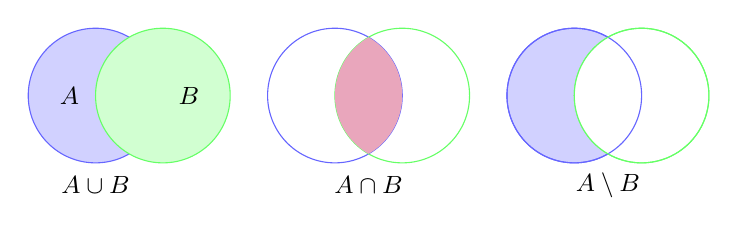
\begin{tikzpicture}[scale=0.95, every node/.style={font=\small}]
\begin{scope}
\draw[fill=blue!18, draw=blue!60] (0,0) circle (0.9);
\draw[fill=green!18, draw=green!60] (0.9,0) circle (0.9);
\node at (0,-1.2) {$A\cup B$};
\node at (-0.35,0) {$A$};
\node at (1.25,0) {$B$};
\end{scope}
\begin{scope}[xshift=3.2cm]
\draw[draw=blue!60] (0,0) circle (0.9);
\draw[draw=green!60] (0.9,0) circle (0.9);
\begin{scope}
\clip (0,0) circle (0.9);
\fill[purple!35] (0.9,0) circle (0.9);
\end{scope}
\node at (0.45,-1.2) {$A\cap B$};
\end{scope}
\begin{scope}[xshift=6.4cm]
\draw[fill=blue!18, draw=blue!60] (0,0) circle (0.9);
\draw[fill=white, draw=green!60] (0.9,0) circle (0.9);
\begin{scope}
\clip (0.9,0) circle (0.9);
\fill[white] (0,0) circle (0.9);
\end{scope}
\draw[draw=blue!60] (0,0) circle (0.9);
\draw[draw=green!60] (0.9,0) circle (0.9);
\node at (0.45,-1.2) {$A\setminus B$};
\end{scope}
\end{tikzpicture}
\end{center}

The formal proof still comes from membership:
\[
x\in A\cap B \quad\text{means}\quad x\in A\text{ and }x\in B.
\]
The diagram helps you guess the identity. The element proof verifies it for arbitrary sets, not just friendly circles on a page.

\begin{trapbox}
False intuition: Venn diagrams prove all set identities. They are excellent intuition for a few sets, but they can hide details about empty sets, indexed families, ambient universes, and arbitrary collections. Use diagrams to see; use definitions to prove.
\end{trapbox}

\subsection{Intervals and common number sets}

Many early examples use subsets of $\R$. The standard intervals are:
\[
(a,b)=\{x\in\R:a<x<b\},
\]
\[
[a,b]=\{x\in\R:a\leq x\leq b\},
\]
\[
(a,b]=\{x\in\R:a<x\leq b\},
\]
\[
[a,b)=\{x\in\R:a\leq x<b\}.
\]

Infinite intervals work similarly:
\[
(a,\infty)=\{x\in\R:x>a\},
\]
\[
(-\infty,b]=\{x\in\R:x\leq b\}.
\]
The symbols $\infty$ and $-\infty$ are not real numbers here. They are notation indicating that the interval has no finite endpoint in that direction.

Some useful number sets:
\[
\N=\text{natural numbers},
\]
\[
\Z=\text{integers},
\]
\[
\Q=\text{rational numbers},
\]
\[
\R=\text{real numbers},
\]
\[
\C=\text{complex numbers}.
\]

Be alert: some authors include $0$ in $\N$, and some do not. If a proof depends on this, say which convention you are using.

Set language makes familiar facts precise:
\[
\N\subseteq\Z\subseteq\Q\subseteq\R\subseteq\C.
\]
Also,
\[
[0,1]\cap[1,2]=\{1\},
\]
while
\[
(0,1)\cap(1,2)=\varnothing.
\]

\begin{historybox}
Intervals are the bridge from elementary set language to analysis and topology. In calculus, intervals are where functions are continuous or differentiable. In topology, intervals generate the usual open sets of the real line. In measure theory, intervals are the first pieces from which length and integration are built.
\end{historybox}

\subsection{Indexed unions and intersections}

Union and intersection are not limited to two sets. If $\{A_i:i\in I\}$ is a family of sets indexed by a set $I$, then
\[
\bigcup_{i\in I}A_i=\{x:\exists i\in I\text{ such that }x\in A_i\},
\]
and
\[
\bigcap_{i\in I}A_i=\{x:\forall i\in I,\ x\in A_i\}.
\]

The quantifiers are the point. Union uses an existential quantifier. Intersection uses a universal quantifier.

Example:
\[
\bigcup_{n\in\N}\left(0,1-\frac1n\right)=(0,1)
\]
if $\N=\{1,2,3,\ldots\}$. The interval for $n=1$ is empty, for $n=2$ is $(0,1/2)$, for $n=3$ is $(0,2/3)$, and so on. Every real number between $0$ and $1$ eventually appears in one of these intervals.

By contrast,
\[
\bigcap_{n\in\N}\left(0,1+\frac1n\right)=(0,1].
\]
Every number in $(0,1]$ lies in all the intervals. A number larger than $1$ eventually gets excluded.

Here is a discrete example. Let
\[
A_n=\{k\in\N:k\geq n\}.
\]
Then
\[
\bigcup_{n\in\N}A_n=\N,
\]
because every natural number is at least $1$. But
\[
\bigcap_{n\in\N}A_n=\varnothing,
\]
because no natural number is at least every natural number.

\begin{trapbox}
When reading indexed unions and intersections, translate them into quantifiers. Most mistakes come from treating ``some index'' and ``every index'' as if they were the same.
\end{trapbox}

\subsection{Cartesian products and ordered pairs}

Sets can be combined by forming ordered pairs. The Cartesian product of $A$ and $B$ is
\[
A\times B=\{(a,b):a\in A\text{ and }b\in B\}.
\]

If
\[
A=\{1,2\},\qquad B=\{x,y,z\},
\]
then
\[
A\times B=\{(1,x),(1,y),(1,z),(2,x),(2,y),(2,z)\}.
\]

Order matters:
\[
(1,x)\neq(x,1)
\]
unless the two coordinates happen to be equal in a context where that comparison even makes sense. Also,
\[
A\times B
\]
is generally not equal to
\[
B\times A.
\]

The plane $\R^2$ is the Cartesian product
\[
\R\times\R.
\]
The space $\R^3$ is
\[
\R\times\R\times\R.
\]

Cartesian products are where set theory starts to feel geometric. A subset of $\R^2$ is a set of points in the plane. A graph of a function is a subset of a Cartesian product. A relation from $A$ to $B$ is a subset of $A\times B$.

This viewpoint will matter when we define functions. A function can be understood as a special kind of relation, hence as a special subset of $A\times B$.

\begin{intuitionbox}
The product $A\times B$ is the set of all possible input-output pairs if the first coordinate must come from $A$ and the second from $B$.
\end{intuitionbox}

\subsection{Partitions and equivalence classes}

A partition of a set $A$ is a way of breaking $A$ into nonempty, nonoverlapping pieces whose union is all of $A$.

\begin{formalbox}
A collection $\mathcal{P}$ of subsets of $A$ is a partition of $A$ if:
\[
\forall P\in\mathcal{P},\ P\neq\varnothing,
\]
\[
\forall P,Q\in\mathcal{P},\ P\neq Q\Rightarrow P\cap Q=\varnothing,
\]
and
\[
\bigcup_{P\in\mathcal{P}}P=A.
\]
\end{formalbox}

Example: the even and odd integers form a partition of $\Z$:
\[
E=\{n\in\Z:n\text{ is even}\},
\]
\[
O=\{n\in\Z:n\text{ is odd}\},
\]
and
\[
\{E,O\}
\]
is a partition of $\Z$.

Partitions connect to equivalence relations. If we define $a\sim b$ to mean that $a$ and $b$ have the same remainder when divided by $3$, then the equivalence classes are
\[
3\Z,\quad 3\Z+1,\quad 3\Z+2.
\]
These three sets partition $\Z$.

This is the first glimpse of quotient constructions. In algebra, quotient groups and quotient rings collect elements into equivalence classes. In topology, quotient spaces glue points together. In software, partitioning appears in hashing, bucketing, grouping records by a key, and classifying states by an invariant.

\begin{historybox}
Cantor's work on sets did not only create a language for collections; it made possible a more flexible way of identifying when two objects should count as the same for a given purpose. Equivalence classes and quotient structures are now central in algebra, topology, geometry, and theoretical computer science.
\end{historybox}

\subsection{A first look at size}

For finite sets, size is counted by the number of elements. We write $|A|$ for the cardinality of $A$. If
\[
A=\{a,b,c\},
\]
then
\[
|A|=3.
\]

For finite sets:
\[
|A\cup B|=|A|+|B|-|A\cap B|.
\]
The subtraction prevents double-counting the overlap.

If $A$ and $B$ are disjoint, meaning $A\cap B=\varnothing$, then
\[
|A\cup B|=|A|+|B|.
\]

For Cartesian products:
\[
|A\times B|=|A||B|
\]
when $A$ and $B$ are finite.

Infinite sets require a deeper idea. Cantor's insight was that two sets have the same size if there is a bijection between them. This means the natural numbers and the even natural numbers have the same infinite size, because
\[
f:\N\to 2\N,\qquad f(n)=2n
\]
matches every natural number with exactly one even natural number and misses no even natural number.

At first that seems impossible. The evens are a proper subset of the naturals. But infinite size does not behave like finite size. This is one of the reasons functions matter so much: they let us compare sets by pairing elements.

\begin{focusbox}
The deep bridge from sets to functions is this: to understand a set, we often study the maps into it, out of it, and between it and other sets.
\end{focusbox}

\subsection{Exercises for sets}

\begin{exercise}
For each pair, decide whether the objects are equal.
\[
\{1,2,3\}\quad\text{and}\quad\{3,2,1,1\},
\]
\[
\{1\}\quad\text{and}\quad 1,
\]
\[
\varnothing\quad\text{and}\quad\{\varnothing\},
\]
\[
\{x\in\Z:x^2=4\}\quad\text{and}\quad\{-2,2\}.
\]
\end{exercise}

\begin{exercise}
Let $A=\{1,2,3,4\}$ and $B=\{3,4,5\}$. Compute $A\cup B$, $A\cap B$, $A\setminus B$, $B\setminus A$, and $\pow(\{1,2\})$.
\end{exercise}

\begin{exercise}
Write each set in set-builder notation:
\[
\{0,2,4,6,8,\ldots\},
\]
\[
(-3,5],
\]
\[
\{1,4,9,16,25,\ldots\}.
\]
State the domain in each case.
\end{exercise}

\begin{exercise}
Let $A_n=(0,1/n)$ for $n\in\N$. Find
\[
\bigcup_{n\in\N}A_n
\quad\text{and}\quad
\bigcap_{n\in\N}A_n.
\]
Explain your answer using quantifiers.
\end{exercise}

\begin{walkbox}
As you move through the day, look for examples of sets: possible passwords, open browser tabs, files in a directory, accepted inputs to a function, rows returned by a query. For each one, ask what membership means.
\end{walkbox}

\section{Set Proofs}

\subsection{The basic method: element chasing}

Most elementary set proofs are element-chasing proofs. This means we prove statements about sets by taking an arbitrary element and following what membership means.

To prove
\[
A\subseteq B,
\]
we prove:
\[
\forall x,\ x\in A\Rightarrow x\in B.
\]
The proof pattern is:

\begin{quote}
Let $x\in A$ be arbitrary. We will show $x\in B$.
\end{quote}

To prove
\[
A=B,
\]
we usually prove both containments:
\[
A\subseteq B\quad\text{and}\quad B\subseteq A.
\]
The proof pattern is:

\begin{quote}
First let $x\in A$ and show $x\in B$. Then let $x\in B$ and show $x\in A$.
\end{quote}

\begin{focusbox}
Set equality is usually proved by two subset proofs.
\end{focusbox}

This is not merely a recipe. It comes from the definition:
\[
A=B\Longleftrightarrow\forall x,\ (x\in A\Longleftrightarrow x\in B).
\]
A biconditional can be proved by proving both directions.

\subsection{Worked proof: intersection is contained in each set}

\begin{theorem}
For all sets $A$ and $B$,
\[
A\cap B\subseteq A
\]
and
\[
A\cap B\subseteq B.
\]
\end{theorem}

\begin{proof}
We prove $A\cap B\subseteq A$. Let $x\in A\cap B$ be arbitrary. By the definition of intersection, $x\in A$ and $x\in B$. In particular, $x\in A$. Therefore $A\cap B\subseteq A$.

The proof that $A\cap B\subseteq B$ is similar. Let $x\in A\cap B$ be arbitrary. Then $x\in A$ and $x\in B$, so in particular $x\in B$. Hence $A\cap B\subseteq B$.
\end{proof}

This proof is short because the theorem is mostly a direct unpacking of definitions. Many early proofs are like this. Do not be disappointed by that. You are learning how definitions move.

\begin{intuitionbox}
If $x$ is in the overlap of $A$ and $B$, then $x$ is certainly in $A$ and certainly in $B$.
\end{intuitionbox}

The formal proof is the disciplined version of that sentence.

\subsection{Worked proof: distributivity}

Set operations distribute over each other in ways that mirror logic.

\begin{theorem}
For all sets $A$, $B$, and $C$,
\[
A\cap(B\cup C)=(A\cap B)\cup(A\cap C).
\]
\end{theorem}

\begin{proof}
We prove equality by proving both containments.

First, let $x\in A\cap(B\cup C)$. Then $x\in A$ and $x\in B\cup C$. Since $x\in B\cup C$, we know $x\in B$ or $x\in C$.

If $x\in B$, then $x\in A$ and $x\in B$, so $x\in A\cap B$. Therefore $x\in (A\cap B)\cup(A\cap C)$.

If $x\in C$, then $x\in A$ and $x\in C$, so $x\in A\cap C$. Therefore $x\in (A\cap B)\cup(A\cap C)$.

In either case, $x\in (A\cap B)\cup(A\cap C)$. Hence
\[
A\cap(B\cup C)\subseteq (A\cap B)\cup(A\cap C).
\]

Conversely, let $x\in (A\cap B)\cup(A\cap C)$. Then $x\in A\cap B$ or $x\in A\cap C$.

If $x\in A\cap B$, then $x\in A$ and $x\in B$. Since $x\in B$, we have $x\in B\cup C$. Thus $x\in A\cap(B\cup C)$.

If $x\in A\cap C$, then $x\in A$ and $x\in C$. Since $x\in C$, we have $x\in B\cup C$. Thus $x\in A\cap(B\cup C)$.

In either case, $x\in A\cap(B\cup C)$. Hence
\[
(A\cap B)\cup(A\cap C)\subseteq A\cap(B\cup C).
\]

Therefore
\[
A\cap(B\cup C)=(A\cap B)\cup(A\cap C).
\]
\end{proof}

Read the proof again and notice the structure. Every step is membership translation:
\[
x\in A\cap(B\cup C)
\]
becomes
\[
x\in A\quad\text{and}\quad (x\in B\text{ or }x\in C).
\]
That is logical distributivity:
\[
P\land(Q\lor R)\Longleftrightarrow(P\land Q)\lor(P\land R).
\]

\subsection{De Morgan's laws}

De Morgan's laws explain how complement interacts with union and intersection. They are among the most useful set identities in analysis, topology, probability, and logic.

\begin{theorem}
Let $A$ and $B$ be subsets of a fixed universe $U$. Then
\[
(A\cup B)^c=A^c\cap B^c
\]
and
\[
(A\cap B)^c=A^c\cup B^c.
\]
\end{theorem}

\begin{proof}
We prove the first identity. Let $x\in U$. Then
\[
x\in(A\cup B)^c
\]
if and only if
\[
x\notin A\cup B.
\]
This holds if and only if it is not true that $x\in A$ or $x\in B$. By De Morgan's law for logic, this is equivalent to
\[
x\notin A\text{ and }x\notin B.
\]
That is equivalent to
\[
x\in A^c\text{ and }x\in B^c,
\]
which is equivalent to
\[
x\in A^c\cap B^c.
\]
Therefore $(A\cup B)^c=A^c\cap B^c$.

The proof of the second identity is similar, using the logical equivalence
\[
\neg(P\land Q)\Longleftrightarrow(\neg P)\lor(\neg Q).
\]
\end{proof}

This proof used a chain of biconditionals rather than separate containment proofs. That is also legitimate. If for every $x$ in the universe we show
\[
x\in S\Longleftrightarrow x\in T,
\]
then $S=T$.

\begin{trapbox}
Do not write $(A\cup B)^c=A^c\cup B^c$. Complement flips union into intersection and intersection into union.
\end{trapbox}

\subsection{Proofs involving the empty set}

The empty set often feels strange because universal statements about it are automatically true. The statement
\[
\forall x\in\varnothing,\ P(x)
\]
is true, because there is no $x\in\varnothing$ that could violate $P$.

This is called vacuous truth. It is not a trick. The implication
\[
x\in\varnothing\Rightarrow P(x)
\]
is true for every $x$, because the premise is always false.

\begin{theorem}
For every set $A$,
\[
\varnothing\subseteq A.
\]
\end{theorem}

\begin{proof}
To show $\varnothing\subseteq A$, we must show that every element of $\varnothing$ is an element of $A$.

Let $x\in\varnothing$ be arbitrary. But there is no such $x$. Therefore there is no counterexample to the statement that every element of $\varnothing$ lies in $A$. Hence $\varnothing\subseteq A$.
\end{proof}

Some readers dislike the sentence ``Let $x\in\varnothing$'' because no such $x$ exists. A more formal version avoids that discomfort:

\begin{proof}
For every object $x$, the implication
\[
x\in\varnothing\Rightarrow x\in A
\]
is true, since $x\in\varnothing$ is false. Therefore $\varnothing\subseteq A$.
\end{proof}

\begin{intuitionbox}
To disprove $\varnothing\subseteq A$, you would need to find an element of $\varnothing$ that is not in $A$. There are no elements of $\varnothing$ to find.
\end{intuitionbox}

\subsection{How to disprove a set statement}

To disprove a universal set identity, find a counterexample. This can mean finding specific sets for which the proposed identity fails, or finding an element that belongs to one side but not the other.

False claim:
\[
A\cup B=A\cap B
\]
for all sets $A$ and $B$.

Counterexample: let
\[
A=\{1\},\qquad B=\{2\}.
\]
Then
\[
A\cup B=\{1,2\}
\]
while
\[
A\cap B=\varnothing.
\]
So the equality fails.

False claim:
\[
A\setminus(B\cup C)=(A\setminus B)\cup(A\setminus C)
\]
for all sets $A$, $B$, and $C$.

Take
\[
A=\{1\},\qquad B=\{1\},\qquad C=\varnothing.
\]
Then
\[
A\setminus(B\cup C)=\varnothing,
\]
but
\[
(A\setminus B)\cup(A\setminus C)=\varnothing\cup\{1\}=\{1\}.
\]
The statement is false.

The correct identity is
\[
A\setminus(B\cup C)=(A\setminus B)\cap(A\setminus C).
\]
This is De Morgan's law in another form.

\begin{trapbox}
When a statement says ``for all sets,'' one small concrete counterexample is enough to disprove it. You do not need to explain all possible failures.
\end{trapbox}

\subsection{Common algebra of sets}

Many set identities resemble algebraic identities:
\[
A\cup B=B\cup A,
\]
\[
A\cap B=B\cap A,
\]
\[
A\cup(B\cup C)=(A\cup B)\cup C,
\]
\[
A\cap(B\cap C)=(A\cap B)\cap C,
\]
\[
A\cup A=A,
\]
\[
A\cap A=A,
\]
\[
A\cup\varnothing=A,
\]
\[
A\cap\varnothing=\varnothing.
\]

These can all be proved by element chasing. For example:

\begin{theorem}
For every set $A$,
\[
A\cup A=A.
\]
\end{theorem}

\begin{proof}
Let $x$ be arbitrary. Then
\[
x\in A\cup A
\]
if and only if
\[
x\in A\text{ or }x\in A,
\]
which is equivalent to $x\in A$. Therefore $A\cup A=A$.
\end{proof}

The corresponding logical law is
\[
P\lor P\Longleftrightarrow P.
\]

There is a useful analogy with Boolean algebra. If we think of a set $A$ as a truth-valued function on a universe $U$, then union corresponds to OR, intersection to AND, and complement to NOT. This is not just analogy. It is a precise algebraic connection.

\begin{historybox}
Boolean algebra, named after George Boole, gave algebraic form to logical operations. Set operations became a natural model of Boolean algebra. This connection is now everywhere: digital circuits, database queries, type systems, probability events, sigma-algebras, and topology all use the same underlying pattern.
\end{historybox}

\subsection{Proof lab: a two-containment proof}

\begin{labbox}
Prove that for all sets $A$, $B$, and $C$,
\[
A\setminus(B\cap C)=(A\setminus B)\cup(A\setminus C).
\]

Before writing the proof, translate membership in each side:
\[
x\in A\setminus(B\cap C)
\]
means
\[
x\in A\quad\text{and}\quad x\notin B\cap C.
\]
The second part means
\[
\text{not }(x\in B\text{ and }x\in C),
\]
which means
\[
x\notin B\quad\text{or}\quad x\notin C.
\]
Now distribute:
\[
x\in A\text{ and }(x\notin B\text{ or }x\notin C).
\]
This is equivalent to
\[
(x\in A\text{ and }x\notin B)\text{ or }(x\in A\text{ and }x\notin C).
\]
That is exactly membership in
\[
(A\setminus B)\cup(A\setminus C).
\]
\end{labbox}

A polished proof could use the above chain directly. A slower proof can split into cases. Both are acceptable. The important habit is to translate the set notation into membership logic.

\subsection{Proof lab: proving a subset of a union}

\begin{labbox}
Prove:
\[
A\subseteq A\cup B.
\]

Proof skeleton:

Let $x\in A$ be arbitrary. Since $x\in A$, it follows that $x\in A$ or $x\in B$. Therefore $x\in A\cup B$. Hence $A\subseteq A\cup B$.
\end{labbox}

This proof may look almost too easy, because the move from $x\in A$ to $x\in A$ or $x\in B$ is a basic logical move:
\[
P\Rightarrow(P\lor Q).
\]
You are allowed to introduce a true OR statement when you already know one side is true.

This little proof appears constantly in larger arguments. For example, in topology, if $U$ is open and $V$ is any open set, then $U\subseteq U\cup V$. In probability, if event $A$ occurs, then event $A\cup B$ occurs. In program analysis, if a state satisfies condition $A$, then it satisfies the broader condition $A$ OR $B$.

\subsection{Proof lab: proving equality of power sets}

\begin{theorem}
For all sets $A$ and $B$,
\[
A\subseteq B\quad\Longleftrightarrow\quad \pow(A)\subseteq\pow(B).
\]
\end{theorem}

\begin{proof}
First assume $A\subseteq B$. We will show $\pow(A)\subseteq\pow(B)$. Let $S\in\pow(A)$ be arbitrary. By definition of power set, $S\subseteq A$. Since $A\subseteq B$, every element of $S$ is an element of $B$. Thus $S\subseteq B$, so $S\in\pow(B)$. Therefore $\pow(A)\subseteq\pow(B)$.

Conversely, assume $\pow(A)\subseteq\pow(B)$. We will show $A\subseteq B$. Since $A\subseteq A$, we have $A\in\pow(A)$. Because $\pow(A)\subseteq\pow(B)$, it follows that $A\in\pow(B)$. By definition of power set, $A\subseteq B$.
\end{proof}

This proof is a good test of level discipline. In the first direction, $S$ is an element of $\pow(A)$, so $S$ is a subset of $A$. In the second direction, $A$ itself is an element of $\pow(A)$.

\begin{trapbox}
When working with $\pow(A)$, remember that its elements are subsets of $A$. If $x\in A$, that does not mean $x\in\pow(A)$. Usually it does not.
\end{trapbox}

\subsection{Set proofs with indexed families}

Indexed unions and intersections require more care because their definitions contain quantifiers.

\begin{theorem}
Let $\{A_i:i\in I\}$ be a family of sets, and let $B$ be a set. Then
\[
B\cap\left(\bigcup_{i\in I}A_i\right)=\bigcup_{i\in I}(B\cap A_i).
\]
\end{theorem}

\begin{proof}
Let $x$ be arbitrary. Then
\[
x\in B\cap\left(\bigcup_{i\in I}A_i\right)
\]
if and only if
\[
x\in B\quad\text{and}\quad x\in\bigcup_{i\in I}A_i.
\]
This is equivalent to
\[
x\in B\quad\text{and}\quad \exists i\in I\text{ such that }x\in A_i.
\]
Since $x\in B$ does not depend on $i$, this is equivalent to
\[
\exists i\in I\text{ such that }x\in B\text{ and }x\in A_i.
\]
That is equivalent to
\[
\exists i\in I\text{ such that }x\in B\cap A_i.
\]
Therefore
\[
x\in\bigcup_{i\in I}(B\cap A_i).
\]
Since this holds for arbitrary $x$, the sets are equal.
\end{proof}

There is a subtle assumption hidden in many informal presentations of indexed intersections: what if the index set $I$ is empty? Different contexts define empty intersections carefully, usually as the whole universe under discussion. For early proof work, most indexed families you meet will have nonempty index sets, but later mathematics cannot ignore the edge case.

\begin{trapbox}
When proving a statement about $\bigcap_{i\in I}A_i$, ask whether $I$ is known to be nonempty. Empty index sets can change the statement.
\end{trapbox}

\subsection{A proof using contradiction}

Some set proofs are cleaner by contradiction.

\begin{theorem}
If $A\subseteq B$ and $B\cap C=\varnothing$, then $A\cap C=\varnothing$.
\end{theorem}

\begin{proof}
Suppose, for contradiction, that $A\cap C\neq\varnothing$. Then there exists $x\in A\cap C$. Hence $x\in A$ and $x\in C$.

Since $A\subseteq B$ and $x\in A$, we have $x\in B$. Therefore $x\in B$ and $x\in C$, so $x\in B\cap C$.

This contradicts $B\cap C=\varnothing$. Therefore $A\cap C=\varnothing$.
\end{proof}

A direct proof is also possible:

\begin{proof}
Let $x\in A\cap C$. Then $x\in A$ and $x\in C$. Since $A\subseteq B$, $x\in B$. Thus $x\in B\cap C$, impossible because $B\cap C=\varnothing$. Hence no such $x$ exists, and $A\cap C=\varnothing$.
\end{proof}

The two proofs are nearly the same. The difference is framing. Contradiction begins by assuming the target fails. Direct proof may show that membership in the target set is impossible.

\subsection{Common traps in set proofs}

\begin{trapbox}
Trap 1: Proving only one containment when equality is required.

If you prove $A\subseteq B$, you have not proved $A=B$. You also need $B\subseteq A$, unless you use a valid biconditional chain.
\end{trapbox}

\begin{trapbox}
Trap 2: Using a diagram as a proof.

Venn diagrams are useful for intuition and counterexample hunting, but they are not usually accepted as complete proofs in rigorous writing. Convert the diagram into element-chasing logic.
\end{trapbox}

\begin{trapbox}
Trap 3: Confusing subset and membership.

The statement $x\in A$ and the statement $x\subseteq A$ are usually about different kinds of objects. The first says $x$ is an element. The second says $x$ is a set whose elements lie in $A$.
\end{trapbox}

\begin{trapbox}
Trap 4: Forgetting the universe when using complement.

The complement of $A$ in $\R$ differs from the complement of $A$ in $\Z$. State the universe or make sure it is already fixed.
\end{trapbox}

\subsection{Exercises for set proofs}

\begin{exercise}
Prove that for all sets $A$ and $B$,
\[
A\cap B\subseteq A\cup B.
\]
\end{exercise}

\begin{exercise}
Prove that for all sets $A$, $B$, and $C$,
\[
A\cup(B\cap C)=(A\cup B)\cap(A\cup C).
\]
\end{exercise}

\begin{exercise}
Prove that for all sets $A$ and $B$,
\[
A\setminus B=A\cap B^c
\]
assuming a fixed universe.
\end{exercise}

\begin{exercise}
Disprove the claim that for all sets $A$, $B$, and $C$,
\[
A\cap(B\setminus C)=(A\cap B)\setminus(A\cap C)
\]
or prove it if it is true.
\end{exercise}

\begin{exercise}
Let $\{A_i:i\in I\}$ be a family of sets. Prove that if $j\in I$, then
\[
\bigcap_{i\in I}A_i\subseteq A_j.
\]
\end{exercise}

\begin{walkbox}
When you see a set identity, do not first ask whether you remember it. Ask what it says about an arbitrary element $x$.
\end{walkbox}

\section{Functions}

\subsection{Functions as disciplined input-output rules}

A function is often introduced as a formula, such as
\[
f(x)=x^2+1.
\]
That is useful, but it is incomplete. A function is not just a formula. A function has a domain, a codomain, and a rule assigning to each element of the domain exactly one element of the codomain.

\begin{formalbox}
A function $f:A\to B$ consists of:
\begin{itemize}
\item a domain $A$,
\item a codomain $B$,
\item an assignment that sends each $a\in A$ to exactly one element $f(a)\in B$.
\end{itemize}
\end{formalbox}

The notation
\[
f:A\to B
\]
means $f$ is a function from $A$ to $B$. If $a\in A$, then $f(a)$ is the value of $f$ at $a$.

The phrase ``exactly one'' is doing real work. A function must be defined for every element of its domain, and it must not assign two different outputs to the same input.

For example,
\[
f:\R\to\R,\qquad f(x)=x^2
\]
is a function. Every real number has exactly one square.

The rule
\[
x\mapsto \pm\sqrt{x}
\]
is not a function from $[0,\infty)$ to $\R$, because most positive inputs have two outputs. We can make functions by choosing one branch:
\[
g:[0,\infty)\to\R,\qquad g(x)=\sqrt{x},
\]
or
\[
h:[0,\infty)\to\R,\qquad h(x)=-\sqrt{x}.
\]

\begin{trapbox}
A formula by itself is not the whole function. The same formula with a different domain or codomain can define a different function.
\end{trapbox}

\subsection{Domain, codomain, and range}

The domain is the set of allowed inputs. The codomain is the set where outputs are declared to live. The range, also called the image of the function, is the set of outputs actually hit.

For
\[
f:\R\to\R,\qquad f(x)=x^2,
\]
the domain is $\R$, the codomain is $\R$, and the range is $[0,\infty)$.

For
\[
g:\R\to[0,\infty),\qquad g(x)=x^2,
\]
the domain is $\R$, the codomain is $[0,\infty)$, and the range is $[0,\infty)$.

The formulas are the same, but the functions are not identical because the codomains differ.

\begin{intuitionbox}
The codomain is the promised output type. The range is what actually appears during execution.
\end{intuitionbox}

Software analogies are helpful but imperfect. A function signature like
\[
\texttt{square: Real -> Real}
\]
declares an input type and output type. The implementation might never return a negative number, but the declared output type still allows one. Similarly, a mathematical codomain may be larger than the range.

This distinction becomes crucial for surjectivity. The function $f:\R\to\R$ given by $f(x)=x^2$ is not surjective. The function $g:\R\to[0,\infty)$ given by $g(x)=x^2$ is surjective. Same formula, different codomain, different property.

\subsection{Functions as relations}

A relation from $A$ to $B$ is a subset of $A\times B$. A function is a relation satisfying two conditions:

\begin{itemize}
\item every $a\in A$ appears as the first coordinate of at least one ordered pair,
\item no $a\in A$ appears as the first coordinate of more than one ordered pair.
\end{itemize}

In other words, $f\subseteq A\times B$ is a function from $A$ to $B$ if for every $a\in A$, there exists exactly one $b\in B$ such that $(a,b)\in f$.

The graph of a function
\[
f:A\to B
\]
is
\[
\Gamma_f=\{(a,f(a)):a\in A\}\subseteq A\times B.
\]

For example, the graph of
\[
f:\R\to\R,\qquad f(x)=x^2
\]
is
\[
\Gamma_f=\{(x,y)\in\R^2:y=x^2\}.
\]

This graph viewpoint is more than a picture. It lets us define functions in very general settings. In set theory, a function can literally be represented as its graph.

\begin{focusbox}
The vertical line test is the geometric version of the ``exactly one output for each input'' rule.
\end{focusbox}

The relation
\[
R=\{(x,y)\in\R^2:y^2=x\}
\]
is not a function $\R\to\R$, because $x=1$ relates to both $y=1$ and $y=-1$. But it can be restricted or reinterpreted to become a function, such as
\[
f:[0,\infty)\to[0,\infty),\qquad f(x)=\sqrt{x}.
\]

\subsection{Equality of functions}

Two functions are equal when they have the same domain, the same codomain, and the same values at every input.

\begin{formalbox}
If $f:A\to B$ and $g:C\to D$, then $f=g$ means:
\[
A=C,\qquad B=D,\qquad \forall x\in A,\ f(x)=g(x).
\]
\end{formalbox}

Some contexts identify functions only by their graphs, in which case codomain may be treated differently. In most proof-writing contexts for functions $A\to B$, the codomain is part of the data.

Example:
\[
f:\R\to\R,\qquad f(x)=x^2,
\]
and
\[
g:\R\to[0,\infty),\qquad g(x)=x^2
\]
are not equal as functions with specified codomains, even though they assign the same formula to each real input.

The functions
\[
p:\R\to\R,\qquad p(x)=(x+1)^2
\]
and
\[
q:\R\to\R,\qquad q(x)=x^2+2x+1
\]
are equal, because their domains and codomains are the same and
\[
(x+1)^2=x^2+2x+1
\]
for every $x\in\R$.

\begin{trapbox}
Do not prove two functions are equal by checking a few inputs. You must prove equality for every input in the domain.
\end{trapbox}

\subsection{Composition}

Composition is the operation of feeding the output of one function into another. If
\[
f:A\to B
\]
and
\[
g:B\to C,
\]
then the composite
\[
g\circ f:A\to C
\]
is defined by
\[
(g\circ f)(a)=g(f(a)).
\]

The order is important. The notation $g\circ f$ means first $f$, then $g$.

Example:
\[
f:\R\to\R,\quad f(x)=x^2,
\]
\[
g:\R\to\R,\quad g(x)=x+1.
\]
Then
\[
(g\circ f)(x)=g(f(x))=g(x^2)=x^2+1,
\]
while
\[
(f\circ g)(x)=f(g(x))=f(x+1)=(x+1)^2.
\]
Usually
\[
g\circ f\neq f\circ g.
\]

Composition is associative:
\[
h\circ(g\circ f)=(h\circ g)\circ f
\]
whenever the domains and codomains match.

\begin{proof}
Let $f:A\to B$, $g:B\to C$, and $h:C\to D$. For any $a\in A$,
\[
\bigl(h\circ(g\circ f)\bigr)(a)=h((g\circ f)(a))=h(g(f(a))).
\]
Also,
\[
\bigl((h\circ g)\circ f\bigr)(a)=(h\circ g)(f(a))=h(g(f(a))).
\]
The two functions have the same domain, codomain, and value at every $a\in A$, so they are equal.
\end{proof}

Composition is the main operation in many parts of mathematics. In linear algebra, matrix multiplication represents composition of linear maps. In abstract algebra, homomorphisms compose. In topology, continuous functions compose. In category theory, composition becomes one of the basic axioms.

\subsection{Identity functions}

For every set $A$, the identity function on $A$ is
\[
\operatorname{id}_A:A\to A,\qquad \operatorname{id}_A(a)=a.
\]

It does nothing, but it does nothing in a very structured way.

If $f:A\to B$, then
\[
f\circ \operatorname{id}_A=f
\]
and
\[
\operatorname{id}_B\circ f=f.
\]

The subscripts matter. The function $\operatorname{id}_A$ has domain and codomain $A$. The function $\operatorname{id}_B$ has domain and codomain $B$.

\begin{proof}
For any $a\in A$,
\[
(f\circ\operatorname{id}_A)(a)=f(\operatorname{id}_A(a))=f(a).
\]
Thus $f\circ\operatorname{id}_A=f$.

Also, for any $a\in A$,
\[
(\operatorname{id}_B\circ f)(a)=\operatorname{id}_B(f(a))=f(a).
\]
Thus $\operatorname{id}_B\circ f=f$.
\end{proof}

Identity functions are the function-world version of neutral elements. Zero is neutral for addition, one is neutral for multiplication, and identity maps are neutral for composition.

\subsection{Restrictions and extensions}

If $f:A\to B$ and $S\subseteq A$, the restriction of $f$ to $S$ is the function
\[
f|_S:S\to B
\]
defined by
\[
f|_S(s)=f(s)
\]
for all $s\in S$.

Example:
\[
f:\R\to\R,\qquad f(x)=x^2.
\]
The restriction
\[
f|_{[0,\infty)}:[0,\infty)\to\R
\]
has the same formula, but only accepts nonnegative inputs.

Restrictions can change important properties. The function $f:\R\to\R$ with $f(x)=x^2$ is not injective, because $f(1)=f(-1)$. But its restriction to $[0,\infty)$ is injective.

An extension goes the other direction. If $g:S\to B$ and $S\subseteq A$, an extension of $g$ to $A$ is a function $f:A\to B$ such that
\[
f|_S=g.
\]

Extensions are central in analysis and topology. A continuous function defined on a dense subset may or may not extend continuously to a larger space. A linear map defined on a basis extends uniquely to a vector space. A local solution to a differential equation may extend only up to a finite time.

\begin{intuitionbox}
Restriction narrows the allowed inputs. Extension fills in values on new inputs while preserving the old behavior.
\end{intuitionbox}

\subsection{Piecewise-defined functions}

A function may be defined by different rules on different parts of its domain:
\[
f:\R\to\R,\qquad
f(x)=
\begin{cases}
x^2,&x\geq0,\\
-x,&x<0.
\end{cases}
\]

This is a valid function because every real number falls into exactly one of the cases.

Piecewise definitions require coverage and consistency:

\begin{itemize}
\item every input in the domain must be covered by at least one case,
\item if an input is covered by multiple cases, the rules must give the same output.
\end{itemize}

Consider:
\[
g:\R\to\R,\qquad
g(x)=
\begin{cases}
0,&x\leq0,\\
1,&x\geq0.
\end{cases}
\]
This is not a well-defined function as written, because $x=0$ falls into both cases and receives two different values.

But
\[
h:\R\to\R,\qquad
h(x)=
\begin{cases}
0,&x<0,\\
1,&x\geq0
\end{cases}
\]
is well-defined.

\begin{trapbox}
For piecewise functions, always check the boundary points. Most mistakes happen where cases overlap or leave a gap.
\end{trapbox}

\subsection{Well-definedness}

To say a function is well-defined means the proposed rule really assigns exactly one valid output to each allowed input.

For ordinary formulas, this can be easy. The function
\[
f:\R\to\R,\qquad f(x)=x^2+1
\]
is well-defined because every real $x$ gives exactly one real number $x^2+1$.

But well-definedness becomes subtle when the input has multiple representations.

Example: define
\[
F:\Q\to\Z
\]
by saying if $q=a/b$ in lowest terms, set
\[
F(q)=a+b.
\]
This is well-defined because every rational number has a unique lowest-terms representation up to multiplying both numerator and denominator by $-1$. If we require $b>0$, then the representation is unique.

But if we define
\[
G:\Q\to\Z,\qquad G(a/b)=a+b
\]
using any representation $a/b$, then it is not well-defined:
\[
\frac12=\frac24,
\]
but
\[
1+2=3
\]
while
\[
2+4=6.
\]
The same rational number would receive different outputs.

Well-definedness is especially important in quotient structures. If elements are equivalence classes, a formula using representatives must not depend on which representative is chosen.

\begin{historybox}
The demand for well-definedness is one of the quiet engines of modern algebra. Quotient groups, quotient rings, vector spaces modulo subspaces, and homology groups all rely on defining operations on equivalence classes without depending on arbitrary representatives.
\end{historybox}

\subsection{Worked proof: a function is well-defined}

Let $\Z_3$ denote the set of congruence classes modulo $3$:
\[
\Z_3=\{[0],[1],[2]\}.
\]
Define
\[
F:\Z_3\to\Z_3,\qquad F([n])=[2n].
\]
We need to check this is well-defined. The input $[n]$ may have many representatives. For example,
\[
[1]=[4]=[-2].
\]
The formula must give the same output no matter which representative is used.

\begin{proof}
Suppose $[n]=[m]$ in $\Z_3$. Then $n\equiv m\pmod 3$, so $3$ divides $n-m$. Therefore $3$ divides $2n-2m=2(n-m)$, hence
\[
2n\equiv 2m\pmod 3.
\]
Thus $[2n]=[2m]$. Therefore $F([n])=[2n]$ is independent of the representative, so $F$ is well-defined.
\end{proof}

Notice the proof did not merely compute three examples. It proved that any two representatives of the same class lead to the same output.

\subsection{Functions in analysis, topology, and algebra}

In analysis, functions are the main objects of study. Continuity, differentiability, integrability, convergence, and boundedness are properties of functions or sequences of functions. A sequence is a function
\[
a:\N\to\R,
\]
usually written $a_n$ instead of $a(n)$.

In topology, continuous functions are the structure-preserving maps. A topological space is a set with a notion of open subsets. A function
\[
f:X\to Y
\]
between topological spaces is continuous if inverse images of open sets are open. This definition may look different from the epsilon-delta definition in calculus, but it is built from the same function and set language.

In algebra, homomorphisms are functions that preserve operations. A group homomorphism
\[
\varphi:G\to H
\]
satisfies
\[
\varphi(ab)=\varphi(a)\varphi(b).
\]
A linear map
\[
T:V\to W
\]
satisfies
\[
T(v+w)=T(v)+T(w)
\]
and
\[
T(cv)=cT(v).
\]

Thus, functions are not merely computational rules. They are how mathematics compares structures.

\begin{focusbox}
In advanced mathematics, objects matter, but maps between objects often matter more.
\end{focusbox}

\subsection{Structure-Preserving Maps: A First Category-Theoretic Hint}

Here is a sentence worth carrying for years:

\begin{quote}
Modern mathematics studies objects by studying the maps that preserve their structure.
\end{quote}

This is the first tiny hint of category theory. You do not need category theory yet, but the perspective is useful immediately.

\begin{center}
\begin{tikzpicture}[
  node distance=1.4cm,
  obj/.style={draw, rounded corners, minimum width=2.5cm, minimum height=0.8cm, fill=blue!5},
  arrow/.style={-{Latex}, thick}
]
\node[obj] (A) {Object $A$};
\node[obj, right=3.0cm of A] (B) {Object $B$};
\draw[arrow] (A) -- node[above] {structure-preserving map} (B);
\node[below=0.55cm of A, text width=2.7cm, align=center] {set, group, space, manifold};
\node[below=0.55cm of B, text width=2.7cm, align=center] {set, group, space, manifold};
\end{tikzpicture}
\end{center}

Different fields choose different structures and different maps:

\begin{longtable}{p{0.22\linewidth}p{0.32\linewidth}p{0.34\linewidth}}
\toprule
Field & Object & Structure-preserving map \\
\midrule
Set theory & sets & functions \\
Linear algebra & vector spaces & linear maps \\
Group theory & groups & homomorphisms \\
Topology & topological spaces & continuous maps \\
Differential geometry & smooth manifolds & smooth maps \\
Algebraic geometry & varieties/schemes & regular morphisms \\
\bottomrule
\end{longtable}

This perspective explains why functions deserve so much attention before Velleman. Functions are not a side topic. They are the roads between mathematical worlds.

\subsection{Exercises for functions}

\begin{exercise}
For each rule, decide whether it defines a function with the stated domain and codomain.
\[
f:\R\to\R,\quad f(x)=\frac1x,
\]
\[
g:\R\setminus\{0\}\to\R,\quad g(x)=\frac1x,
\]
\[
h:[0,\infty)\to\R,\quad h(x)=\pm\sqrt{x},
\]
\[
k:\R\to[0,\infty),\quad k(x)=x^2.
\]
\end{exercise}

\begin{exercise}
Let $f:\R\to\R$ be given by $f(x)=2x+3$, and let $g:\R\to\R$ be given by $g(x)=x^2$. Compute $f\circ g$ and $g\circ f$.
\end{exercise}

\begin{exercise}
Prove that if $f:A\to B$, then $f\circ\operatorname{id}_A=f$ and $\operatorname{id}_B\circ f=f$.
\end{exercise}

\begin{exercise}
Let $f:\R\to\R$ be $f(x)=|x|$. Find a restriction of $f$ that is injective. Find a codomain restriction that makes the resulting function surjective.
\end{exercise}

\begin{exercise}
Define $F:\Z_5\to\Z_5$ by $F([n])=[n+2]$. Prove that $F$ is well-defined.
\end{exercise}

\begin{walkbox}
When you see a function formula, ask three questions before doing algebra: what is the domain, what is the codomain, and what values are actually hit?
\end{walkbox}

\section{Injective, Surjective, and Bijective Functions}

\subsection{Why these three words matter}

Injective, surjective, and bijective describe how a function matches inputs to outputs.

Informally:

\begin{itemize}
\item injective means different inputs never collide,
\item surjective means every target output is hit,
\item bijective means both: every target output is hit exactly once.
\end{itemize}

These ideas are the beginning of mathematical comparison. If two finite sets have the same number of elements, there is a bijection between them. Cantor extended this idea to infinite sets: two sets have the same cardinality if there is a bijection between them.

\begin{historybox}
Cantor's theory of cardinality used bijections to compare infinite sets. This led to surprising results: $\N$ and $\Z$ have the same cardinality, $\N$ and $\Q$ have the same cardinality, but $\N$ and $\R$ do not. The language of injective, surjective, and bijective maps is the language behind those comparisons.
\end{historybox}

These properties are also everywhere in algebra and topology. An isomorphism is usually a bijective structure-preserving map whose inverse also preserves structure. A homeomorphism is a bijective continuous map with continuous inverse. A change of coordinates is useful when it is invertible. A database key acts like an injective identifier. A parser is unambiguous when different source structures do not collapse to the same parse result.

\subsection{Injective functions}

\begin{formalbox}
A function $f:A\to B$ is injective, or one-to-one, if
\[
\forall a_1,a_2\in A,\ f(a_1)=f(a_2)\Rightarrow a_1=a_2.
\]
\end{formalbox}

This says collisions do not happen. If two inputs produce the same output, then they were not really two different inputs.

Equivalent contrapositive:
\[
a_1\neq a_2\Rightarrow f(a_1)\neq f(a_2).
\]

Example:
\[
f:\R\to\R,\qquad f(x)=2x+3
\]
is injective. If
\[
f(x_1)=f(x_2),
\]
then
\[
2x_1+3=2x_2+3,
\]
so
\[
x_1=x_2.
\]

Example:
\[
g:\R\to\R,\qquad g(x)=x^2
\]
is not injective, because
\[
g(1)=1=g(-1)
\]
but
\[
1\neq -1.
\]

The proof pattern for injectivity is:

\begin{quote}
Assume $f(a_1)=f(a_2)$. Use algebra or structure to prove $a_1=a_2$.
\end{quote}

To disprove injectivity:

\begin{quote}
Find $a_1\neq a_2$ such that $f(a_1)=f(a_2)$.
\end{quote}

\begin{trapbox}
Do not prove injectivity by showing that one output has one input. You must show that every output has at most one input, or equivalently that no two different inputs collide.
\end{trapbox}

\subsection{Surjective functions}

\begin{formalbox}
A function $f:A\to B$ is surjective, or onto, if
\[
\forall b\in B,\ \exists a\in A\text{ such that }f(a)=b.
\]
\end{formalbox}

Surjectivity is about the codomain. Every element of the codomain must be hit.

Example:
\[
f:\R\to\R,\qquad f(x)=2x+3
\]
is surjective. Let $y\in\R$ be arbitrary. We need $x\in\R$ such that
\[
2x+3=y.
\]
Solving gives
\[
x=\frac{y-3}{2}.
\]
This is real, and
\[
f\left(\frac{y-3}{2}\right)=2\left(\frac{y-3}{2}\right)+3=y.
\]
So $f$ is surjective.

Example:
\[
g:\R\to\R,\qquad g(x)=x^2
\]
is not surjective, because $-1\in\R$ but no real $x$ satisfies
\[
x^2=-1.
\]

But
\[
h:\R\to[0,\infty),\qquad h(x)=x^2
\]
is surjective. Given $y\in[0,\infty)$, choose $x=\sqrt y$. Then $h(x)=y$.

\begin{focusbox}
Surjectivity can change when the codomain changes, even if the formula does not.
\end{focusbox}

The proof pattern for surjectivity is:

\begin{quote}
Let $b\in B$ be arbitrary. Construct $a\in A$ such that $f(a)=b$.
\end{quote}

\subsection{Bijective functions}

\begin{formalbox}
A function $f:A\to B$ is bijective if it is both injective and surjective.
\end{formalbox}

Equivalently, for every $b\in B$, there exists exactly one $a\in A$ such that
\[
f(a)=b.
\]

Example:
\[
f:\R\to\R,\qquad f(x)=2x+3
\]
is bijective. We already proved it is injective and surjective.

Example:
\[
g:\R\to[0,\infty),\qquad g(x)=x^2
\]
is surjective but not injective.

Example:
\[
h:[0,\infty)\to[0,\infty),\qquad h(x)=x^2
\]
is bijective. It is injective on $[0,\infty)$ because if $x_1^2=x_2^2$ and $x_1,x_2\geq0$, then $x_1=x_2$. It is surjective because every $y\geq0$ has $x=\sqrt y\geq0$ with $x^2=y$.

Bijective functions are exactly the functions that have inverse functions in the ordinary two-sided sense.

\subsection{Inverse functions}

If $f:A\to B$ is bijective, then its inverse is the function
\[
f^{-1}:B\to A
\]
defined by
\[
f^{-1}(b)=\text{the unique }a\in A\text{ such that }f(a)=b.
\]

The word unique depends on injectivity. The existence depends on surjectivity.

If $f$ is not surjective, some $b\in B$ has no preimage, so $f^{-1}(b)$ cannot be defined for every $b\in B$.

If $f$ is not injective, some $b\in B$ has multiple preimages, so $f^{-1}(b)$ is ambiguous.

For a bijection,
\[
f^{-1}\circ f=\operatorname{id}_A
\]
and
\[
f\circ f^{-1}=\operatorname{id}_B.
\]

\begin{proof}
Let $a\in A$. Since $f(a)$ is the output corresponding to $a$, the unique input mapped to $f(a)$ is $a$. Thus
\[
f^{-1}(f(a))=a.
\]
Therefore $f^{-1}\circ f=\operatorname{id}_A$.

Let $b\in B$. By definition, $f^{-1}(b)$ is the unique $a\in A$ with $f(a)=b$. Therefore
\[
f(f^{-1}(b))=b.
\]
Thus $f\circ f^{-1}=\operatorname{id}_B$.
\end{proof}

\begin{trapbox}
Do not confuse inverse functions with inverse images. The notation $f^{-1}$ is used for both, but the meanings differ. An inverse function exists only for bijections. Inverse images of sets exist for every function.
\end{trapbox}

\subsection{Left inverses and right inverses}

There is a useful relationship between injectivity, surjectivity, and one-sided inverses.

A function $g:B\to A$ is a left inverse of $f:A\to B$ if
\[
g\circ f=\operatorname{id}_A.
\]
This means $g$ undoes $f$ after $f$ is applied.

A function $h:B\to A$ is a right inverse of $f:A\to B$ if
\[
f\circ h=\operatorname{id}_B.
\]
This means $h$ chooses a preimage for each element of $B$.

\begin{theorem}
If $f:A\to B$ has a left inverse, then $f$ is injective.
\end{theorem}

\begin{proof}
Suppose $g:B\to A$ satisfies $g\circ f=\operatorname{id}_A$. Let $a_1,a_2\in A$ and assume $f(a_1)=f(a_2)$. Applying $g$ to both sides gives
\[
g(f(a_1))=g(f(a_2)).
\]
Since $g\circ f=\operatorname{id}_A$,
\[
a_1=a_2.
\]
Thus $f$ is injective.
\end{proof}

\begin{theorem}
If $f:A\to B$ has a right inverse, then $f$ is surjective.
\end{theorem}

\begin{proof}
Suppose $h:B\to A$ satisfies $f\circ h=\operatorname{id}_B$. Let $b\in B$ be arbitrary. Choose $a=h(b)\in A$. Then
\[
f(a)=f(h(b))=b.
\]
Therefore every $b\in B$ is hit, so $f$ is surjective.
\end{proof}

The converses require mild set-theoretic care in full generality, especially for arbitrary surjections and choice functions. In most elementary contexts, an injective function can be given a left inverse after choosing default values, and a surjective function has right inverses by choosing one preimage for each target.

\subsection{Composition and injectivity}

\begin{theorem}
If $f:A\to B$ and $g:B\to C$ are injective, then $g\circ f:A\to C$ is injective.
\end{theorem}

\begin{proof}
Let $a_1,a_2\in A$ and assume
\[
(g\circ f)(a_1)=(g\circ f)(a_2).
\]
Then
\[
g(f(a_1))=g(f(a_2)).
\]
Since $g$ is injective,
\[
f(a_1)=f(a_2).
\]
Since $f$ is injective,
\[
a_1=a_2.
\]
Therefore $g\circ f$ is injective.
\end{proof}

The proof shows how information travels backward through an injective composition. Equality at the end forces equality one step earlier, then one step earlier again.

\begin{theorem}
If $g\circ f$ is injective, then $f$ is injective.
\end{theorem}

\begin{proof}
Let $a_1,a_2\in A$ and assume $f(a_1)=f(a_2)$. Applying $g$ gives
\[
g(f(a_1))=g(f(a_2)),
\]
so
\[
(g\circ f)(a_1)=(g\circ f)(a_2).
\]
Since $g\circ f$ is injective, $a_1=a_2$. Therefore $f$ is injective.
\end{proof}

Notice that this theorem says nothing about $g$ being injective. The composite may be injective even if $g$ fails to be injective outside the range of $f$.

\subsection{Composition and surjectivity}

\begin{theorem}
If $f:A\to B$ and $g:B\to C$ are surjective, then $g\circ f:A\to C$ is surjective.
\end{theorem}

\begin{proof}
Let $c\in C$ be arbitrary. Since $g$ is surjective, there exists $b\in B$ such that
\[
g(b)=c.
\]
Since $f$ is surjective, there exists $a\in A$ such that
\[
f(a)=b.
\]
Then
\[
(g\circ f)(a)=g(f(a))=g(b)=c.
\]
Therefore $g\circ f$ is surjective.
\end{proof}

\begin{theorem}
If $g\circ f$ is surjective, then $g$ is surjective.
\end{theorem}

\begin{proof}
Let $c\in C$ be arbitrary. Since $g\circ f$ is surjective, there exists $a\in A$ such that
\[
(g\circ f)(a)=c.
\]
Let $b=f(a)\in B$. Then
\[
g(b)=g(f(a))=c.
\]
Thus every $c\in C$ is hit by $g$, so $g$ is surjective.
\end{proof}

Again, this says nothing about $f$ being surjective. The composite might hit all of $C$ even if $f$ misses part of $B$, as long as the missed part is not needed by $g$ to hit $C$.

\subsection{Finite sets and counting}

For finite sets, injectivity and surjectivity are connected by counting.

\begin{theorem}
Let $A$ and $B$ be finite sets with $|A|=|B|$. For a function $f:A\to B$, the following are equivalent:
\[
f\text{ is injective},
\]
\[
f\text{ is surjective},
\]
\[
f\text{ is bijective}.
\]
\end{theorem}

The intuition is simple. If $A$ and $B$ have the same finite number of elements, then a collision among inputs forces some output to be missed. Conversely, if some output is missed, then two inputs must collide.

This principle is sometimes called the pigeonhole principle in disguise.

\begin{proof}
Assume $A$ and $B$ are finite with $|A|=|B|=n$.

If $f$ is injective, then the $n$ different elements of $A$ produce $n$ different outputs in $B$. Since $B$ has exactly $n$ elements, every element of $B$ is hit. Thus $f$ is surjective.

If $f$ is surjective, then every element of $B$ is hit. Since $B$ has $n$ elements, the range has $n$ elements. If two different elements of $A$ had the same output, then $n$ inputs would produce fewer than $n$ outputs, contradicting that the range has $n$ elements. Thus $f$ is injective.

Therefore injectivity and surjectivity are equivalent, and either one implies bijectivity.
\end{proof}

For infinite sets, this theorem is false. The function
\[
f:\N\to\N,\qquad f(n)=n+1
\]
is injective but not surjective if $\N=\{1,2,3,\ldots\}$, because $1$ is not hit. The function
\[
g:\N\to\N,\qquad
g(1)=1,\quad g(n)=n-1\text{ for }n\geq2
\]
is surjective but not injective, because $g(1)=g(2)=1$.

\begin{focusbox}
Finite intuition is useful, but infinite sets often break it. Cantor's work begins exactly at that breaking point.
\end{focusbox}

\subsection{Proof lab: proving bijectivity}

\begin{labbox}
Prove that
\[
f:\R\setminus\{1\}\to\R\setminus\{2\},\qquad f(x)=\frac{2x+1}{x-1}
\]
is bijective.

For injectivity, assume
\[
\frac{2x_1+1}{x_1-1}=\frac{2x_2+1}{x_2-1}.
\]
Cross-multiply:
\[
(2x_1+1)(x_2-1)=(2x_2+1)(x_1-1).
\]
Expand and simplify. The terms $2x_1x_2$ cancel, leaving
\[
-2x_1+x_2-1=-2x_2+x_1-1,
\]
so
\[
3x_2=3x_1,
\]
and $x_1=x_2$.

For surjectivity, let $y\in\R\setminus\{2\}$. Solve
\[
y=\frac{2x+1}{x-1}.
\]
Then
\[
y(x-1)=2x+1,
\]
so
\[
x(y-2)=y+1.
\]
Since $y\neq2$, define
\[
x=\frac{y+1}{y-2}.
\]
Check that $x\neq1$, because $x=1$ would imply $y+1=y-2$, impossible. Then compute $f(x)=y$.
\end{labbox}

This lab illustrates the standard algebraic pattern. To prove surjectivity, solve $y=f(x)$ for $x$ in terms of $y$, then check that the proposed $x$ is actually in the domain.

\subsection{Common traps}

\begin{trapbox}
Trap 1: Ignoring the codomain.

The function $x\mapsto x^2$ is not simply ``surjective'' or ``not surjective'' until its codomain is specified.
\end{trapbox}

\begin{trapbox}
Trap 2: Trying to prove surjectivity by starting with an arbitrary input.

For surjectivity, start with an arbitrary element of the codomain, then find a preimage in the domain.
\end{trapbox}

\begin{trapbox}
Trap 3: Trying to prove injectivity by solving $f(x)=y$.

That may help, but the direct injectivity pattern is to assume $f(x_1)=f(x_2)$ and prove $x_1=x_2$.
\end{trapbox}

\begin{trapbox}
Trap 4: Calling every inverse-looking notation an inverse function.

For a general function $f$, the notation $f^{-1}(S)$ usually means inverse image of a set $S$, not an inverse function value.
\end{trapbox}

\subsection{Exercises for injective, surjective, bijective}

\begin{exercise}
For each function, determine whether it is injective, surjective, bijective, or none.
\[
f:\R\to\R,\quad f(x)=x^3,
\]
\[
g:\R\to\R,\quad g(x)=e^x,
\]
\[
h:\R\to(0,\infty),\quad h(x)=e^x,
\]
\[
p:\Z\to\Z,\quad p(n)=n+1.
\]
\end{exercise}

\begin{exercise}
Prove that if $f:A\to B$ and $g:B\to C$ are bijective, then $g\circ f:A\to C$ is bijective.
\end{exercise}

\begin{exercise}
Give an example of functions $f:A\to B$ and $g:B\to C$ such that $g\circ f$ is injective but $g$ is not injective.
\end{exercise}

\begin{exercise}
Give an example of functions $f:A\to B$ and $g:B\to C$ such that $g\circ f$ is surjective but $f$ is not surjective.
\end{exercise}

\begin{exercise}
Let $A$ be a finite set. Prove that a function $f:A\to A$ is injective if and only if it is surjective.
\end{exercise}

\begin{walkbox}
Look at a login system, a file path, or a database primary key. Ask which maps should be injective, which should be surjective, and which should not be either.
\end{walkbox}

\section{Images and Inverse Images}

\subsection{From points to sets}

So far, $f(a)$ has meant the output of a function at one input. Images and inverse images extend this pointwise language to sets.

If
\[
f:A\to B
\]
and $S\subseteq A$, the image of $S$ under $f$ is the set of outputs reached from inputs in $S$:
\[
f(S)=\{f(s):s\in S\}.
\]
Equivalently,
\[
f(S)=\{b\in B:\exists s\in S\text{ such that }f(s)=b\}.
\]

If $T\subseteq B$, the inverse image, or preimage, of $T$ under $f$ is
\[
f^{-1}(T)=\{a\in A:f(a)\in T\}.
\]

\begin{focusbox}
Images move subsets of the domain forward. Inverse images move subsets of the codomain backward.
\end{focusbox}

Example:
\[
f:\R\to\R,\qquad f(x)=x^2.
\]
If
\[
S=[-2,3],
\]
then
\[
f(S)=[0,9].
\]
If
\[
T=[1,4],
\]
then
\[
f^{-1}(T)=[-2,-1]\cup[1,2].
\]

Notice that $f^{-1}(T)$ is defined even though $f$ is not bijective. This is inverse image, not inverse function.

\subsection{Image of a set}

The image of $S\subseteq A$ under $f:A\to B$ is
\[
f(S)=\{b\in B:\exists s\in S,\ f(s)=b\}.
\]

The existential quantifier is important. An element $b$ belongs to $f(S)$ if at least one element of $S$ maps to $b$.

Example:
\[
f:\Z\to\Z,\qquad f(n)=n^2.
\]
If
\[
S=\{-2,-1,0,1,2\},
\]
then
\[
f(S)=\{0,1,4\}.
\]
Different inputs can collapse to the same output. Images do not remember multiplicity.

If
\[
S=2\Z
\]
is the set of even integers, then
\[
f(S)=\{4k^2:k\in\Z\}.
\]
This is the set of squares of even integers.

The image of the whole domain is the range:
\[
f(A)=\operatorname{range}(f).
\]

\begin{trapbox}
Do not assume $f(S)=\{f(s)\}$ for one unspecified $s$. The image of a set contains outputs from all elements of the set.
\end{trapbox}

\subsection{Inverse image of a set}

The inverse image of $T\subseteq B$ under $f:A\to B$ is
\[
f^{-1}(T)=\{a\in A:f(a)\in T\}.
\]

This definition has no existential ambiguity. It asks which inputs land inside $T$.

Example:
\[
f:\R\to\R,\qquad f(x)=x^2.
\]
Then
\[
f^{-1}(\{4\})=\{-2,2\},
\]
\[
f^{-1}((-\infty,0))=\varnothing,
\]
\[
f^{-1}([0,1])=[-1,1].
\]

For a constant function
\[
c:A\to B,\qquad c(a)=b_0,
\]
we have
\[
c^{-1}(T)=
\begin{cases}
A,&b_0\in T,\\
\varnothing,&b_0\notin T.
\end{cases}
\]

Inverse images are one of the most important constructions in all of mathematics because they behave especially well with set operations.

\begin{intuitionbox}
The inverse image of $T$ is the set of all inputs that pass the test ``does the output lie in $T$?''
\end{intuitionbox}

In software terms, if $f$ is a function and $T$ is a predicate on outputs, then $f^{-1}(T)$ is the predicate on inputs obtained by composing: accept $a$ if $T(f(a))$ is true.

\subsection{Images of unions and intersections}

Images preserve unions exactly:
\[
f(S\cup T)=f(S)\cup f(T).
\]

\begin{proof}
Let $b\in f(S\cup T)$. Then there exists $a\in S\cup T$ such that $f(a)=b$. Since $a\in S\cup T$, either $a\in S$ or $a\in T$. If $a\in S$, then $b\in f(S)$. If $a\in T$, then $b\in f(T)$. Thus $b\in f(S)\cup f(T)$.

Conversely, let $b\in f(S)\cup f(T)$. Then $b\in f(S)$ or $b\in f(T)$. If $b\in f(S)$, there exists $s\in S$ such that $f(s)=b$. Since $s\in S\cup T$, $b\in f(S\cup T)$. The case $b\in f(T)$ is similar. Therefore $f(S\cup T)=f(S)\cup f(T)$.
\end{proof}

Images do not generally preserve intersections exactly. We always have
\[
f(S\cap T)\subseteq f(S)\cap f(T),
\]
but equality can fail.

Example:
\[
f:\R\to\R,\qquad f(x)=x^2,
\]
\[
S=(-\infty,0],\qquad T=[0,\infty).
\]
Then
\[
S\cap T=\{0\},
\]
so
\[
f(S\cap T)=\{0\}.
\]
But
\[
f(S)=[0,\infty)
\]
and
\[
f(T)=[0,\infty),
\]
so
\[
f(S)\cap f(T)=[0,\infty).
\]
Equality fails.

The reason is collision. A value can be in both $f(S)$ and $f(T)$ because it is hit by one input from $S$ and a different input from $T$.

\begin{theorem}
If $f:A\to B$ is injective, then for all $S,T\subseteq A$,
\[
f(S\cap T)=f(S)\cap f(T).
\]
\end{theorem}

\begin{proof}
We already know $f(S\cap T)\subseteq f(S)\cap f(T)$ for every function.

For the reverse containment, let $b\in f(S)\cap f(T)$. Then $b\in f(S)$ and $b\in f(T)$. So there exist $s\in S$ and $t\in T$ such that
\[
f(s)=b=f(t).
\]
Since $f$ is injective, $s=t$. Therefore this common element lies in both $S$ and $T$, so $s\in S\cap T$. Hence
\[
b=f(s)\in f(S\cap T).
\]
Thus $f(S)\cap f(T)\subseteq f(S\cap T)$, and equality follows.
\end{proof}

\subsection{Inverse images and set operations}

Inverse images preserve unions, intersections, and complements exactly.

\begin{theorem}
Let $f:A\to B$, and let $S,T\subseteq B$. Then
\[
f^{-1}(S\cup T)=f^{-1}(S)\cup f^{-1}(T),
\]
\[
f^{-1}(S\cap T)=f^{-1}(S)\cap f^{-1}(T),
\]
and
\[
f^{-1}(B\setminus S)=A\setminus f^{-1}(S).
\]
\end{theorem}

\begin{proof}
We prove the first identity. Let $a\in A$. Then
\[
a\in f^{-1}(S\cup T)
\]
if and only if
\[
f(a)\in S\cup T.
\]
This is equivalent to
\[
f(a)\in S\text{ or }f(a)\in T.
\]
That is equivalent to
\[
a\in f^{-1}(S)\text{ or }a\in f^{-1}(T),
\]
which is equivalent to
\[
a\in f^{-1}(S)\cup f^{-1}(T).
\]
Thus
\[
f^{-1}(S\cup T)=f^{-1}(S)\cup f^{-1}(T).
\]

The intersection proof is the same with ``and'' replacing ``or.'' For complements:
\[
a\in f^{-1}(B\setminus S)
\]
if and only if
\[
f(a)\in B\setminus S,
\]
which means
\[
f(a)\notin S.
\]
That is equivalent to
\[
a\notin f^{-1}(S),
\]
so
\[
a\in A\setminus f^{-1}(S).
\]
Therefore
\[
f^{-1}(B\setminus S)=A\setminus f^{-1}(S).
\]
\end{proof}

This exact preservation is why topology defines continuity using inverse images. If open sets in $Y$ can be pulled back to open sets in $X$, then the function respects the topological structure.

\begin{historybox}
The inverse-image definition of continuity emerged from the abstraction of analysis into topology. In calculus, continuity is often described by limits and epsilons. In topology, a function $f:X\to Y$ is continuous when $f^{-1}(U)$ is open in $X$ for every open set $U$ in $Y$. This definition works in spaces where distance may not even be present.
\end{historybox}

\subsection{Direct and inverse images under composition}

Images and inverse images behave naturally with composition.

Let
\[
f:A\to B,\qquad g:B\to C.
\]
If $S\subseteq A$, then
\[
(g\circ f)(S)=g(f(S)).
\]

If $T\subseteq C$, then
\[
(g\circ f)^{-1}(T)=f^{-1}(g^{-1}(T)).
\]

\begin{proof}
For the image formula, let $c\in(g\circ f)(S)$. Then there exists $s\in S$ such that
\[
(g\circ f)(s)=c.
\]
That means
\[
g(f(s))=c.
\]
Since $f(s)\in f(S)$, we have $c\in g(f(S))$. The reverse containment follows by unwinding the same definitions.

For inverse images, let $a\in A$. Then
\[
a\in(g\circ f)^{-1}(T)
\]
if and only if
\[
(g\circ f)(a)\in T.
\]
This means
\[
g(f(a))\in T.
\]
That is equivalent to
\[
f(a)\in g^{-1}(T),
\]
which is equivalent to
\[
a\in f^{-1}(g^{-1}(T)).
\]
\end{proof}

The inverse image formula reverses the order:
\[
(g\circ f)^{-1}=f^{-1}\circ g^{-1}
\]
as operations on subsets. This is the same order reversal familiar from inverse functions and matrix products.

\subsection{The relationship between a set and its image-preimage}

For $S\subseteq A$, compare $S$ with
\[
f^{-1}(f(S)).
\]
Every element of $S$ lands in $f(S)$, so
\[
S\subseteq f^{-1}(f(S)).
\]
But equality can fail. If $f$ collapses points outside $S$ onto values hit by $S$, those outside points also appear in the preimage.

Example:
\[
f:\R\to\R,\qquad f(x)=x^2,
\]
and
\[
S=\{1\}.
\]
Then
\[
f(S)=\{1\},
\]
but
\[
f^{-1}(f(S))=f^{-1}(\{1\})=\{-1,1\}.
\]

If $f$ is injective, then equality holds:
\[
f^{-1}(f(S))=S.
\]

\begin{proof}
We already know $S\subseteq f^{-1}(f(S))$. For the reverse containment, let $a\in f^{-1}(f(S))$. Then $f(a)\in f(S)$. So there exists $s\in S$ such that
\[
f(a)=f(s).
\]
Since $f$ is injective, $a=s$. Therefore $a\in S$. Hence
\[
f^{-1}(f(S))\subseteq S.
\]
\end{proof}

For $T\subseteq B$, compare $T$ with
\[
f(f^{-1}(T)).
\]
Every element of $f(f^{-1}(T))$ lies in $T$, so
\[
f(f^{-1}(T))\subseteq T.
\]
But equality can fail if $T$ contains elements not hit by $f$.

Example:
\[
f:\R\to\R,\qquad f(x)=x^2,
\]
and
\[
T=\{-1,1\}.
\]
Then
\[
f^{-1}(T)=\{-1,1\},
\]
so
\[
f(f^{-1}(T))=\{1\}\subsetneq T.
\]

If $f$ is surjective, then equality holds for all $T\subseteq B$:
\[
f(f^{-1}(T))=T.
\]

\subsection{Images, inverse images, and injectivity/surjectivity}

The previous subsection gives useful characterizations.

\begin{theorem}
A function $f:A\to B$ is injective if and only if for every $S\subseteq A$,
\[
f^{-1}(f(S))=S.
\]
\end{theorem}

\begin{proof}
We already proved the forward direction.

Conversely, assume $f^{-1}(f(S))=S$ for every $S\subseteq A$. We show $f$ is injective. Suppose $f(a_1)=f(a_2)$. Let $S=\{a_1\}$. Since $f(a_2)=f(a_1)$, we have
\[
a_2\in f^{-1}(f(S)).
\]
By the assumed equality,
\[
f^{-1}(f(S))=S=\{a_1\}.
\]
Thus $a_2=a_1$. Therefore $f$ is injective.
\end{proof}

\begin{theorem}
A function $f:A\to B$ is surjective if and only if for every $T\subseteq B$,
\[
f(f^{-1}(T))=T.
\]
\end{theorem}

\begin{proof}
Assume $f$ is surjective. We already know $f(f^{-1}(T))\subseteq T$. For the reverse containment, let $t\in T$. Since $f$ is surjective, there exists $a\in A$ such that $f(a)=t$. Since $t\in T$, we have $a\in f^{-1}(T)$. Therefore $t=f(a)\in f(f^{-1}(T))$.

Conversely, assume $f(f^{-1}(T))=T$ for every $T\subseteq B$. Let $b\in B$. Take $T=\{b\}$. Then
\[
f(f^{-1}(\{b\}))=\{b\}.
\]
In particular, the left side is nonempty, so there exists $a\in f^{-1}(\{b\})$. Thus $f(a)=b$. Therefore $f$ is surjective.
\end{proof}

These theorems show that injectivity and surjectivity can be read as statements about how well image and inverse image undo each other.

\subsection{Images and inverse images in topology and analysis}

Continuity in topology is built from inverse images:
\[
f:X\to Y\text{ is continuous}\quad\Longleftrightarrow\quad f^{-1}(U)\text{ is open in }X\text{ for every open }U\subseteq Y.
\]

Why inverse images rather than images? Because inverse images preserve unions and intersections exactly. Topologies are defined by closure under arbitrary unions and finite intersections. If inverse images preserve those operations, the definition behaves cleanly.

Images of open sets do not generally remain open under continuous functions. For example,
\[
f:\R\to\R,\qquad f(x)=x^2
\]
is continuous, but
\[
f((-1,1))=[0,1),
\]
which is not open in $\R$.

In measure theory and probability, inverse images are also essential. A random variable is a function
\[
X:\Omega\to\R.
\]
An event like
\[
\{\omega\in\Omega:X(\omega)\leq 3\}
\]
is the inverse image
\[
X^{-1}((-\infty,3]).
\]
This is how statements about numerical outcomes become events in the sample space.

In analysis, level sets are inverse images:
\[
f^{-1}(\{c\})=\{x:f(x)=c\}.
\]
These appear in optimization, implicit function theory, differential geometry, and partial differential equations.

\begin{historybox}
The language of images and inverse images helped unify analysis, topology, geometry, and probability. The same notation describes the range of a function, the preimage of an open set, the event determined by a random variable, and the fiber of a map in geometry.
\end{historybox}

\subsection{Software analogies}

Suppose a program has a function
\[
\texttt{status: User -> Status}.
\]
If $S$ is a set of users, then $\texttt{status}(S)$ is the set of statuses appearing among those users.

If $T$ is a set of statuses, then $\texttt{status}^{-1}(T)$ is the set of users whose status lies in $T$.

For example, if
\[
T=\{\texttt{active},\texttt{trial}\},
\]
then
\[
\texttt{status}^{-1}(T)
\]
is the set of users whose status is active or trial.

Database queries often use inverse-image thinking. A filter such as

\begin{verbatim}
WHERE status IN ('active', 'trial')
\end{verbatim}

selects the preimage of a subset of possible statuses under the status field.

Hashing gives another example. A hash function
\[
h:\text{Keys}\to\text{Buckets}
\]
maps many possible keys to a smaller set of buckets. The inverse image of a bucket is the set of keys that land in that bucket. Collisions are exactly the reason those inverse images can have more than one element.

\begin{intuitionbox}
An inverse image is a pullback of a condition. A condition on outputs becomes a condition on inputs.
\end{intuitionbox}

\subsection{Proof lab: inverse images preserve arbitrary unions}

\begin{labbox}
Let $f:A\to B$, and let $\{T_i:i\in I\}$ be a family of subsets of $B$. Prove
\[
f^{-1}\left(\bigcup_{i\in I}T_i\right)=\bigcup_{i\in I}f^{-1}(T_i).
\]

Start with arbitrary $a\in A$:
\[
a\in f^{-1}\left(\bigcup_{i\in I}T_i\right)
\]
if and only if
\[
f(a)\in\bigcup_{i\in I}T_i.
\]
This means
\[
\exists i\in I\text{ such that }f(a)\in T_i.
\]
That is equivalent to
\[
\exists i\in I\text{ such that }a\in f^{-1}(T_i),
\]
which means
\[
a\in\bigcup_{i\in I}f^{-1}(T_i).
\]
\end{labbox}

The corresponding intersection identity is
\[
f^{-1}\left(\bigcap_{i\in I}T_i\right)=\bigcap_{i\in I}f^{-1}(T_i),
\]
with the existential quantifier replaced by a universal quantifier.

\subsection{Common traps}

\begin{trapbox}
Trap 1: Treating $f^{-1}(T)$ as requiring an inverse function.

Inverse images exist for every function $f:A\to B$ and every subset $T\subseteq B$.
\end{trapbox}

\begin{trapbox}
Trap 2: Forgetting that $f(S)$ is a subset of the codomain, while $f^{-1}(T)$ is a subset of the domain.

Always ask which side of the function the set lives on.
\end{trapbox}

\begin{trapbox}
Trap 3: Assuming images preserve intersections.

Only the inclusion $f(S\cap T)\subseteq f(S)\cap f(T)$ holds for every function. Equality needs extra hypotheses, such as injectivity.
\end{trapbox}

\begin{trapbox}
Trap 4: Assuming $f(f^{-1}(T))=T$ for every $T$.

This equality holds for all $T\subseteq B$ exactly when $f$ is surjective. In general, the left side is only the part of $T$ that $f$ actually hits.
\end{trapbox}

\subsection{Exercises for images and inverse images}

\begin{exercise}
Let $f:\R\to\R$ be $f(x)=x^2$. Compute:
\[
f([-3,2]),\qquad f^{-1}([4,9]),\qquad f^{-1}((-1,1)),\qquad f(\{-2,0,2\}).
\]
\end{exercise}

\begin{exercise}
Let $f:A\to B$ and let $S,T\subseteq A$. Prove
\[
f(S\cup T)=f(S)\cup f(T).
\]
Then give an example showing that
\[
f(S\cap T)=f(S)\cap f(T)
\]
can fail.
\end{exercise}

\begin{exercise}
Let $f:A\to B$ and let $U,V\subseteq B$. Prove
\[
f^{-1}(U\setminus V)=f^{-1}(U)\setminus f^{-1}(V).
\]
\end{exercise}

\begin{exercise}
Let $f:A\to B$ and $g:B\to C$. Prove that for every $T\subseteq C$,
\[
(g\circ f)^{-1}(T)=f^{-1}(g^{-1}(T)).
\]
\end{exercise}

\begin{exercise}
Prove that $f:A\to B$ is injective if and only if for all subsets $S,T\subseteq A$,
\[
f(S\cap T)=f(S)\cap f(T).
\]
\end{exercise}

\begin{exercise}
Let $X:\Omega\to\R$ be a function. Express the set
\[
\{\omega\in\Omega:1<X(\omega)\leq 5\}
\]
as an inverse image of a subset of $\R$.
\end{exercise}

\begin{walkbox}
When a theorem talks about a subset of the codomain, try pulling it back by inverse image. When it talks about a subset of the domain, try pushing it forward by image. Notice which direction preserves more structure.
\end{walkbox}
